% =====================================================================
% ARTIGO -- Tema 38: Evolução multiobjetivo: custo e tempo de entrega
% Formato SBC (coluna única, A4, Times 12pt) -- baseado no modelo-tcc-sbc.tex
% Compile: pdflatex artigo.tex (2x). No Overleaf: envie este .tex + pasta figuras/.
% Trechos entre [colchetes] devem ser preenchidos pelo grupo.
% =====================================================================
\documentclass[a4paper,12pt]{article}

\usepackage[utf8]{inputenc}
\usepackage[T1]{fontenc}
\usepackage[brazilian]{babel}
\usepackage{times}
\usepackage[a4paper,top=3.5cm,left=3cm,right=3cm,bottom=2.5cm]{geometry}
\usepackage{graphicx}
\usepackage{url}
\usepackage{amsmath,amssymb}
\usepackage{booktabs}
\usepackage{titlesec}
\usepackage[bf,sf,footnotesize,indent]{caption}
% Citações no estilo SBC/ementa: [Autor Ano] e Autor [Ano]
\usepackage[authoryear,square]{natbib}
\setcitestyle{aysep={},yysep={;}}
\setlength{\bibsep}{6pt}
\setlength{\bibhang}{0.5cm}

% Regra da disciplina: 1º parágrafo da seção SEM recuo; demais com 1,27 cm.
% (por isso o pacote indentfirst do modelo original foi retirado)
\setlength{\parindent}{1.27cm}
\setlength{\parskip}{6pt}
\flushbottom

\titleformat{\section}{\fontsize{13}{15}\bfseries}{\thesection.}{1em}{}
\titleformat{\subsection}{\fontsize{12}{14}\bfseries}{\thesubsection.}{1em}{}
\titleformat{\subsubsection}{\fontsize{12}{14}\bfseries\itshape}{\thesubsubsection.}{1em}{}
\titlespacing*{\section}{0pt}{12pt}{6pt}
\titlespacing*{\subsection}{0pt}{10pt}{4pt}

\renewcommand{\captionfont}{\sffamily\footnotesize\bfseries}
\setlength{\captionmargin}{0.8cm}
\captionsetup{labelsep=period}

\newenvironment{resumo}{%
  \list{}{\advance\topsep by6pt\relax
    \leftmargin=0.8cm
    \labelwidth=0pt
    \listparindent=0pt
    \itemindent\listparindent
    \rightmargin\leftmargin}\item[\hskip\labelsep\bfseries\itshape Resumo.]\itshape}%
  {\endlist}

\renewenvironment{abstract}{%
  \list{}{\advance\topsep by6pt\relax
    \leftmargin=0.8cm
    \labelwidth=0pt
    \listparindent=0pt
    \itemindent\listparindent
    \rightmargin\leftmargin}\item[\hskip\labelsep\bfseries\itshape Abstract.]\itshape}%
  {\endlist}

\begin{document}
\pagestyle{empty}
\begin{center}
  {\fontsize{16}{20}\selectfont\bfseries Evolução Multiobjetivo no Roteamento de Entregas: Custo e Tempo de Entrega ao Mesmo Tempo com NSGA-II}\\[4pt]
  {\fontsize{14}{18}\selectfont\bfseries Multi-Objective Evolution for Delivery Routing: Cost and Delivery Time at Once with NSGA-II}\\[12pt]
  {\normalsize\bfseries Enzo Figueiredo Feitosa$^{1}$, Mateus Henrique de Araújo Santos$^{1}$, Pedro Carvalho$^{1}$,\\ Luiz Henrique$^{1}$, Anthony Yuri Feitosa França$^{1}$, Guilherme Santos$^{1}$}\\[6pt]
  {\footnotesize\itshape Professor: Sérgio Santana -- Disciplina: Machine Learning e Data Science}\\[4pt]
  {\normalsize
    $^{1}$Curso de Sistemas de Informação -- Universidade Tiradentes (UNIT) -- Aracaju/SE\\{}
    \footnotesize\texttt{enzo.figueiredo@souunit.com.br, mateus.henrique05@souunit.com.br,\\
    pedro.gcarvalho@souunit.com.br, luiz.hsilva@souunit.com.br,\\
    anthony.yuri@souunit.com.br, guilherme.santos1102@souunit.com.br}
  }
\end{center}
\vspace{12pt}
\begin{resumo}
Empresas de entrega querem baixo custo e prazo curto, objetivos que se opõem, e otimizar uma soma ponderada dos dois devolve uma só resposta, que esconde as alternativas. Este trabalho aplica o NSGA-II a um problema sintético de roteamento com 50 clientes e até 8 veículos, minimizando o custo diário e o tempo médio de entrega, e o compara com a soma ponderada em 30 repetições. Com o mesmo orçamento de avaliações, o NSGA-II obteve hipervolume de 0,851, contra 0,140. Com onze vezes mais avaliações, a soma ponderada chegou a 0,882, mas ofereceu 7,5 alternativas por execução, contra 57,1 do NSGA-II. A frente obtida permite ao gestor escolher a solução por orçamento, por prazo ou pelo ponto de joelho.
\end{resumo}
\noindent\textbf{Palavras-chave:} otimização multiobjetivo, NSGA-II, frente de Pareto, roteamento de veículos, soma ponderada.

\vspace{6pt}

\begin{abstract}
Delivery companies want low cost and short lead times, two conflicting goals, and optimizing a weighted sum of both returns a single answer that hides the alternatives. This work applies NSGA-II to a synthetic routing problem with 50 customers and up to 8 vehicles, minimizing daily cost and mean delivery time, and compares it with the weighted-sum method over 30 runs. Under the same evaluation budget, NSGA-II reached a hypervolume of 0.851, versus 0.140. With eleven times more evaluations, the weighted sum reached 0.882, but offered 7.5 alternatives per run, against 57.1 for NSGA-II. The resulting front lets the manager pick a solution by budget, by deadline or by the knee point.
\end{abstract}
\noindent\textbf{Keywords:} multi-objective optimization, NSGA-II, Pareto front, vehicle routing, weighted sum.

\vspace{18pt}

\section{Introdução}\label{sec:intro}
\noindent No Brasil, o custo logístico deve chegar a 15,5\% do PIB em 2025, dos quais 8,5 pontos percentuais correspondem ao transporte, segundo levantamento do ILOS divulgado por \citep{mundolog2025}. Para uma transportadora ou um e-commerce, cada quilômetro rodado e cada veículo na rua pesam no resultado, ao mesmo tempo em que o cliente espera entregas cada vez mais rápidas. O gestor enfrenta, portanto, dois objetivos que se opõem: reduzir o custo da operação e reduzir o tempo até a entrega.

O conflito é estrutural: a forma mais barata de atender um conjunto de clientes costuma ser concentrar as entregas em poucos veículos com rotas longas, e a mais rápida é dividi-los entre muitos veículos, o que aumenta o custo fixo da frota e a quilometragem. Não há, em geral, uma solução melhor nos dois critérios, e sim um conjunto de soluções de compromisso, a \emph{frente de Pareto}, em que melhorar um objetivo exige piorar o outro \citep{miettinen1999,deb2001}.

Na prática, é comum atribuir pesos ao custo e ao tempo e otimizar a soma ponderada \citep{marler2004}. Essa estratégia exige escolher os pesos \emph{antes} de conhecer as alternativas, devolve uma única resposta por combinação de pesos e, como mostraram \citet{das1997}, não alcança soluções em trechos não convexos da frente. Algoritmos evolutivos multiobjetivo, como o NSGA-II \citep{deb2002}, evoluem uma população inteira e devolvem, em uma única execução, uma aproximação da frente.

O objetivo deste trabalho é avaliar o NSGA-II como apoio à decisão entre custo e tempo de entrega em um problema de roteamento de veículos. Especificamente, busca-se: (i) modelar um problema sintético de roteamento com dois objetivos; (ii) obter a frente de Pareto com o NSGA-II; (iii) compará-la com a soma ponderada, sob o mesmo orçamento computacional e sob um orçamento onze vezes maior; e (iv) ilustrar a escolha de uma solução por critérios de negócio. A Seção \ref{sec:fund} apresenta a fundamentação; a Seção \ref{sec:metodo}, a metodologia; a Seção \ref{sec:impl}, a implementação; a Seção \ref{sec:res}, os resultados; e a Seção \ref{sec:conc}, as conclusões.


\section{Fundamentação Teórica}\label{sec:fund}

\subsection{Otimização multiobjetivo e dominância de Pareto}\label{sec:pareto}
\noindent Um problema multiobjetivo com $M$ objetivos a minimizar busca soluções $\mathbf{x}$ que minimizem o vetor $\mathbf{F}(\mathbf{x}) = (f_1(\mathbf{x}), \ldots, f_M(\mathbf{x}))$. As soluções são comparadas pela relação de \emph{dominância} \citep{miettinen1999,deb2001}: $\mathbf{x}$ domina $\mathbf{y}$ ($\mathbf{x} \prec \mathbf{y}$) quando não é pior em nenhum objetivo e é estritamente melhor em pelo menos um:

\begin{equation}
\mathbf{x} \prec \mathbf{y} \iff f_i(\mathbf{x}) \le f_i(\mathbf{y})\;\; \forall i \in \{1,\ldots,M\} \;\;\text{e}\;\; \exists j : f_j(\mathbf{x}) < f_j(\mathbf{y}).
\label{eq:dom}
\end{equation}
Uma solução que nenhuma outra domina é \emph{Pareto-ótima}; a imagem dessas soluções no espaço dos objetivos é a \emph{frente de Pareto}. Com dois objetivos, a frente é uma curva no plano custo $\times$ tempo, de leitura simples para o tomador de decisão.


\subsection{Algoritmos genéticos e o NSGA-II}\label{sec:nsga}
\noindent Algoritmos genéticos melhoram uma população de soluções ao longo de gerações por seleção, cruzamento e mutação \citep{holland1975,goldberg1989} e, por trabalharem com populações, adequam-se a problemas em que se deseja um conjunto de soluções \citep{coello2007}. O NSGA-II \citep{deb2002} junta pais e filhos a cada geração e os ordena em frentes sucessivas por \emph{ordenação não dominada}: a primeira frente reúne as soluções que ninguém domina, a segunda, as dominadas apenas pela primeira, e assim por diante. A nova população é preenchida frente a frente, o que garante elitismo, e o desempate usa a \emph{distância de aglomeração}, que favorece soluções em regiões menos povoadas e preserva a diversidade. A ordenação custa $O(MN^2)$ por geração, sendo $N$ o tamanho da população.


\subsection{Soma ponderada e hipervolume}\label{sec:sp}
\noindent A soma ponderada minimiza $\sum_i w_i \bar{f}_i(\mathbf{x})$, com objetivos normalizados $\bar{f}_i$ e pesos $w_i \ge 0$ que somam um \citep{marler2004}. É simples, mas exige uma execução por vetor de pesos, alcança apenas as soluções da parte convexa da frente (soluções \emph{suportadas}) e, com pesos uniformemente espaçados, tende a concentrar as soluções em poucas regiões \citep{das1997}.

Para comparar frentes, é preciso medir ao mesmo tempo convergência e diversidade. O \emph{hipervolume} \citep{zitzler1999} mede a área do espaço dos objetivos dominada pelo conjunto de soluções e limitada por um ponto de referência; quanto maior, melhor. É um dos poucos indicadores unários compatíveis com a dominância: se um conjunto domina outro, seu hipervolume é maior \citep{zitzler2003}.


\subsection{Trabalhos relacionados}\label{sec:rel}
\noindent O roteamento de veículos foi formulado por \citet{dantzig1959} e é NP-difícil, o que motiva o uso de metaheurísticas \citep{toth2014}. \citet{potvin2009} revisa algoritmos evolutivos para o problema, com destaque para representações por permutação. Na versão multiobjetivo, \citet{jozefowiez2008} classificam os trabalhos pelos objetivos considerados (distância, número de veículos, equilíbrio de carga, janelas de tempo) e apontam os algoritmos evolutivos como a abordagem mais frequente. \citet{garcia2010} incluem o tempo de entrega como objetivo, ao lado do número de rotas e da distância, e relatam resultados superiores aos do NSGA-II com um algoritmo próprio, que depois aprimoram com uma medida de similaridade entre soluções \citep{garcia2011}. Enquanto esses estudos buscam superar o estado da arte em instâncias de referência, o foco aqui é o apoio à decisão: mostrar, em uma instância controlada, o que o gestor ganha ao receber uma frente em vez de uma única solução.


\section{Metodologia}\label{sec:metodo}

\subsection{Base de dados sintética}\label{sec:base}
\noindent Conforme a delimitação do tema, foi usado um problema sintético, o que permite controlar o cenário e reproduzir os resultados. Foram gerados 50 clientes com coordenadas uniformes em um quadrado de 100 km $\times$ 100 km (semente 42) e um depósito no centro; as distâncias são euclidianas. A frota é homogênea, com até $K_{\max} = 8$ veículos que saem do depósito e retornam ao fim da rota, sem restrição de capacidade, como na entrega de encomendas pequenas. Os demais parâmetros, de ordem de grandeza plausível, estão na Tabela \ref{tab:param}. Não houve pré-processamento, pois os dados já são gerados no formato do modelo.

\begin{table}[!htb]
  \centering
  \caption{Parâmetros do cenário e dos algoritmos.}
  \label{tab:param}
  \small
  \begin{tabular}{ll}
    \toprule
    Parâmetro & Valor \\
    \midrule
    Clientes / frota máxima & 50 / 8 veículos \\
    Velocidade média / parada por cliente & 40 km/h / 10 min \\
    Custo fixo por veículo / custo por km & R\$~250,00 por dia / R\$~2,50 \\
    População / gerações & 100 / 500 (50.000 avaliações) \\
    Cruzamento / mutação & OX, taxa 0,9 / inversão, taxa 0,6 \\
    Pesos da soma ponderada & $w \in \{0; 0{,}1; \ldots; 1\}$ (11 pesos) \\
    Repetições independentes & 30 (sementes 1 a 30) \\
    \bottomrule
  \end{tabular}
\end{table}

\subsection{Modelo e objetivos}\label{sec:modelo}
\noindent Uma solução é um conjunto de rotas $r_1, \ldots, r_K$, com $1 \le K \le K_{\max}$, em que cada cliente aparece uma única vez. Sendo $c_F$ o custo fixo por veículo, $c_D$ o custo por km e $D$ a distância total (com retorno ao depósito), o primeiro objetivo é o custo diário $f_1$. O segundo, $f_2$, é o tempo médio de entrega: a média, sobre os $n = 50$ clientes, do instante $t_j$ em que o veículo chega ao cliente $j$, contado da saída do depósito e incluindo as paradas anteriores:

\begin{equation}
f_1 = c_F \cdot K + c_D \cdot D, \qquad f_2 = \frac{1}{n}\sum_{j=1}^{n} t_j.
\label{eq:obj}
\end{equation}
Um único veículo minimiza o custo fixo, mas o último cliente só é atendido no fim de uma rota longa; usar todos os veículos reduz o tempo médio, mas multiplica o custo fixo e as idas e voltas ao depósito.


\subsection{Representação, operadores e abordagens comparadas}\label{sec:repr}
\noindent Cada solução é uma permutação de $n + K_{\max} - 1 = 57$ genes: os valores 0 a 49 são clientes e os valores 50 a 56 são \emph{separadores} que encerram uma rota e iniciam a próxima. Rotas vazias são descartadas, de modo que o número de veículos emerge da evolução. Toda permutação é válida, o que permite usar o cruzamento por ordem (OX) \citep{davis1985}, que preserva a ordem relativa dos genes dos pais, e a mutação por inversão, que inverte um trecho do cromossomo e pode reordenar uma rota ou mover clientes entre rotas. Indivíduos duplicados são eliminados.

Três abordagens foram comparadas, com os mesmos operadores, população de 100 e a mesma semente em cada repetição. O \emph{NSGA-II} executa 500 gerações (50.000 avaliações). A \emph{SP-total} executa um algoritmo genético mono-objetivo para cada um dos 11 pesos, com 45 gerações cada, totalizando o mesmo orçamento. A \emph{SP-11x} usa 500 gerações por peso (550.000 avaliações) e verifica se as conclusões se mantêm sem limite de orçamento para a soma ponderada. Nas duas, minimiza-se $w \bar{f}_1 + (1-w)\bar{f}_2$, com $\bar{f}_i = (f_i - f_i^{\min})/(f_i^{\max} - f_i^{\min})$ e limites estimados pelas execuções extremas ($w = 1$ e $w = 0$) \citep{marler2004}; das 11 soluções, mantêm-se as não dominadas.


\subsection{Métricas e protocolo de avaliação}\label{sec:metricas}
\noindent Cada abordagem foi executada 30 vezes, com média e desvio padrão reportados. As métricas são: (i) o hipervolume, com objetivos normalizados pela frente de referência (união não dominada de todas as soluções encontradas) e ponto de referência $(1{,}1; 1{,}1)$; (ii) o número de soluções não dominadas oferecidas ao gestor; (iii) os melhores custo e tempo alcançados; e (iv) a maior lacuna, isto é, a maior distância normalizada entre soluções vizinhas da frente. As diferenças foram avaliadas pelo teste de Mann-Whitney \citep{mann1947}, bilateral, com significância de 5\%.

Para ilustrar a decisão, tomou-se a execução do NSGA-II de hipervolume mediano e aplicaram-se três regras: (a) \emph{orçamento}, a solução mais rápida com custo de até R\$~3.000,00 por dia; (b) \emph{prazo}, a mais barata com tempo médio de até 3,0 h; e (c) \emph{ponto de joelho}, a de maior distância à reta que liga os extremos da frente normalizada, região em que pequenas melhoras em um objetivo passam a custar grandes pioras no outro e que costuma ser preferida pelos decisores \citep{branke2004}.


\section{Implementação e Experimentos}\label{sec:impl}
\noindent O experimento foi implementado em Python 3.13 com a biblioteca pymoo 0.6.2 \citep{blank2020}, que fornece o NSGA-II, o algoritmo genético mono-objetivo, os operadores de permutação e o hipervolume; NumPy 2.5 foi usado na avaliação vetorizada da população, SciPy 1.18 no teste estatístico e Matplotlib 3.11 nas figuras. Na avaliação, cada separador é tratado como uma passagem pelo depósito, em que o tempo acumulado é zerado, o que dispensa laços sobre as rotas. A execução ocorreu em ambiente Linux, com processador Intel Xeon de 2,1 GHz e dois processos paralelos, no ambiente da ferramenta de IA indicada na declaração ao final do artigo; cada repetição completa levou em média 79 s, a maior parte gasta pela SP-11x. A análise, as figuras e a conferência das tabelas foram refeitas em um computador pessoal com Windows 11 e as mesmas versões das bibliotecas, com valores idênticos. Todos os valores das Tabelas \ref{tab:metricas} e \ref{tab:gestor} e das figuras foram produzidos pela execução do programa: o script \emph{experimento.py} gera os dados brutos das 30 repetições, \emph{analise.py} calcula as métricas e as figuras, e \emph{verificar\_tabelas.py} reconstrói as tabelas a partir desses dados e confere cada um de seus valores com o texto do artigo. Uma segunda execução completa, feita do zero, reproduziu os mesmos valores. Código, semente e resultados brutos estão disponíveis no repositório do sistema: \url{https://github.com/pedrocarvalho-13/evolucao-multiobjetivo-entregas}.


\section{Resultados e Discussão}\label{sec:res}

\subsection{Comparação quantitativa}\label{sec:quant}
\noindent A Tabela \ref{tab:metricas} resume as métricas nas 30 repetições, e a Figura \ref{fig:box} mostra a dispersão do hipervolume e do número de soluções.

\begin{table}[!htb]
  \centering
  \caption{Métricas nas 30 repetições (média $\pm$ desvio padrão). Custo e tempo mínimos referem-se à melhor solução de cada frente em cada objetivo.}
  \label{tab:metricas}
  \small
  \begin{tabular}{lccc}
    \toprule
    Métrica & NSGA-II & SP-total & SP-11x \\
    \midrule
    Avaliações por repetição & 50.000 & $\approx$ 49.500 & 550.000 \\
    Hipervolume & 0,851 $\pm$ 0,043 & 0,140 $\pm$ 0,031 & 0,882 $\pm$ 0,022 \\
    Nº de soluções não dominadas & 57,1 $\pm$ 14,6 & 7,2 $\pm$ 1,3 & 7,5 $\pm$ 0,7 \\
    Custo mínimo (R\$~) & 2.103 $\pm$ 151 & 3.644 $\pm$ 169 & 1.687 $\pm$ 36 \\
    Tempo médio mínimo (h) & 1,85 $\pm$ 0,06 & 2,90 $\pm$ 0,13 & 1,96 $\pm$ 0,06 \\
    Maior lacuna (normalizada) & 0,479 $\pm$ 0,230 & 0,911 $\pm$ 0,384 & 0,592 $\pm$ 0,027 \\
    \bottomrule
  \end{tabular}
\end{table}
\begin{figure}[!htb]
  \centering
  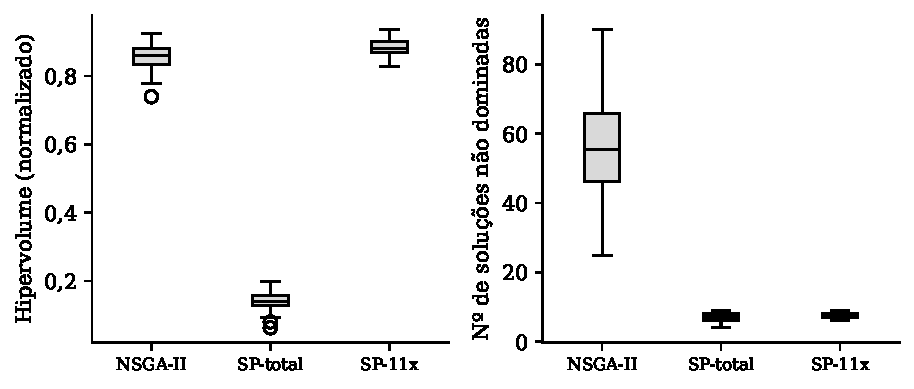
\includegraphics[width=0.74\linewidth]{figuras/fig_boxplot.pdf}
  \caption{Distribuição do hipervolume (à esquerda) e do número de soluções não dominadas (à direita) nas 30 repetições.}
  \label{fig:box}
\end{figure}
Com o mesmo orçamento de avaliações, o NSGA-II foi muito superior à soma ponderada: hipervolume médio de 0,851, contra 0,140 da SP-total ($p = 3{,}0\times 10^{-11}$). A SP-total reinicia a busca para cada peso e dispõe de apenas 45 gerações por execução, insuficientes para organizar rotas de 50 clientes, enquanto o NSGA-II usa uma única população, em que boas sequências de clientes encontradas para uma região da frente são aproveitadas, por cruzamento, nas demais. A Figura \ref{fig:conv} mostra que o NSGA-II supera o hipervolume final da SP-total antes de 10.000 avaliações, menos de um quinto do orçamento.

\begin{figure}[!htb]
  \centering
  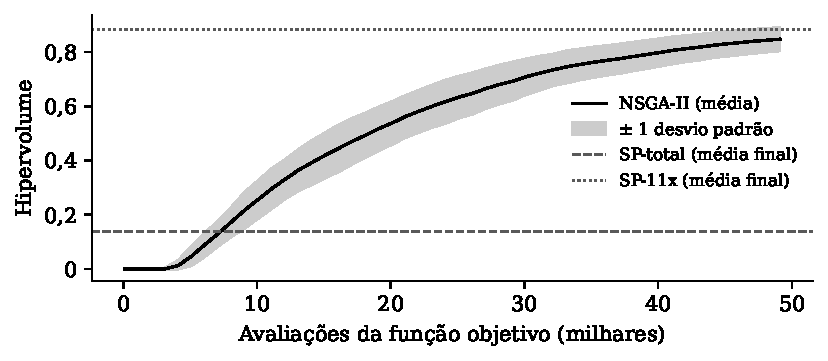
\includegraphics[width=0.68\linewidth]{figuras/fig_convergencia.pdf}
  \caption{Hipervolume da população do NSGA-II ao longo das avaliações (média e desvio padrão em 30 repetições) e valores finais médios da soma ponderada.}
  \label{fig:conv}
\end{figure}
Com onze vezes mais avaliações, a SP-11x obteve hipervolume ligeiramente maior que o do NSGA-II (0,882, diferença de cerca de 0,03; $p = 0{,}002$). A vantagem se concentra no extremo de menor custo: a execução com $w = 1$ dedica 50.000 avaliações a um só compromisso e encontra rotas de um veículo mais curtas (custo mínimo médio de R\$~1.687, contra R\$~2.103). No extremo oposto, o NSGA-II alcançou tempos menores (1,85 h contra 1,96 h). Como a curva da Figura \ref{fig:conv} ainda cresce ao final, um orçamento maior provavelmente reduziria essa diferença, hipótese não testada aqui.

A diferença mais marcante está no número de alternativas: o NSGA-II entregou em média 57,1 soluções não dominadas por execução, cerca de 7,6 vezes mais que a SP-11x ($p = 1{,}7\times 10^{-11}$), que, por construção, guarda uma solução por peso e nunca passa de 11; parte dessa diferença vem, portanto, do próprio desenho da comparação. A maior lacuna, porém, não diferiu de forma significativa ($p = 0{,}773$): as frentes do NSGA-II são densas na região central, mas, em algumas repetições, não chegam ao extremo de menor custo, o que explica a alta variabilidade dessa métrica.


\subsection{Frente de Pareto obtida}\label{sec:frente}
\noindent A Figura \ref{fig:frentes} mostra a frente do NSGA-II na repetição de hipervolume mediano (semente 24, 74 soluções) e as soluções da soma ponderada na mesma repetição. Partindo da solução mais barata, pequenos aumentos de custo trazem grandes reduções do tempo médio, até um ponto a partir do qual cada hora economizada custa muito mais. As soluções da SP-11x ficam próximas da frente, mas espaçadas e por vezes agrupadas em torno dos mesmos valores, como previsto por \citet{das1997} para pesos uniformes; as da SP-total ficam longe dela.

\begin{figure}[!htb]
  \centering
  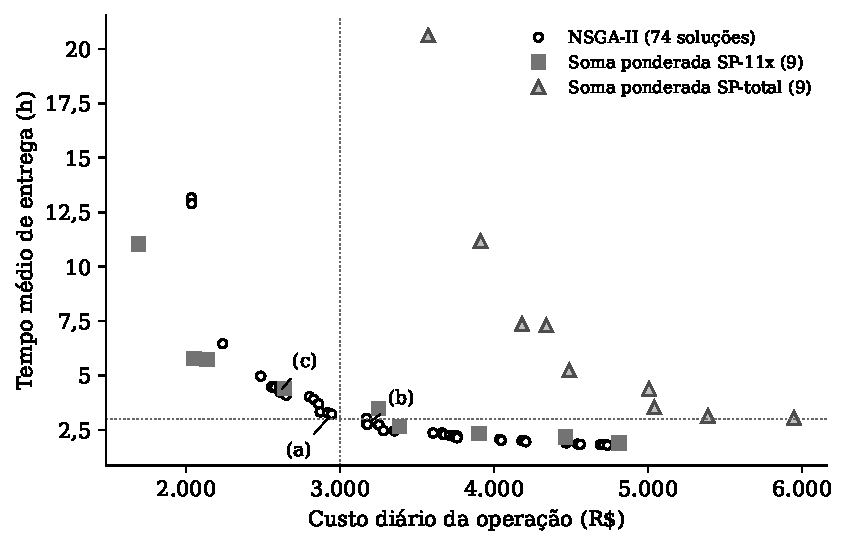
\includegraphics[width=0.74\linewidth]{figuras/fig_frentes.pdf}
  \caption{Frente do NSGA-II na execução de hipervolume mediano e soluções da soma ponderada na mesma repetição. As linhas pontilhadas marcam o orçamento e o prazo do gestor; (a), (b) e (c) são as soluções escolhidas.}
  \label{fig:frentes}
\end{figure}
Um resultado que reforça o argumento do tema é a proporção de soluções \emph{suportadas}, isto é, que minimizam alguma soma ponderada. Calculada com 2.001 pesos dentro da própria frente, ela foi de apenas 19\% nas frentes do NSGA-II. Essa frente, porém, é uma aproximação: em média, 31\% de suas soluções são dominadas por alguma solução da SP-11x na mesma repetição. Tomando como referência a união das frentes das três abordagens, 61\% das soluções do NSGA-II continuam não dominadas e não são suportadas: estão em trechos não convexos da melhor frente conhecida e, se pertencerem à frente ótima, não seriam devolvidas por nenhuma escolha de pesos, por mais execuções que se fizessem \citep{das1997}. Elas não são necessariamente melhores, mas ficam invisíveis para quem usa apenas a soma ponderada.


\subsection{Escolha da solução pelo gestor}\label{sec:gestor}
\noindent Com a frente em mãos, a decisão deixa de ser a escolha prévia de pesos abstratos e passa a ser a escolha entre opções concretas (Tabela \ref{tab:gestor}). Com teto de R\$~3.000,00 por dia (regra a), o gestor obtém tempo médio de 3,22 h com 4 veículos. Exigindo prazo médio de até 3,0 h (regra b), a solução mais barata usa 5 veículos e custa R\$~3.174. O ponto de joelho (regra c), com 3 veículos, reduz o tempo médio em 68\% em relação à solução mais barata, com aumento de custo de 28\%; a partir dele, chegar ao tempo mínimo exige custo 82\% maior para reduzir o tempo em mais 58\%. Esses percentuais tomam como referência o extremo de menor custo do NSGA-II, que, nessa repetição, é dominado pela solução mais barata da SP-11x (R\$~1.692; 11,03 h), coerente com a vantagem da soma ponderada nesse extremo discutida na Seção \ref{sec:quant}.

\begin{table}[!htb]
  \centering
  \caption{Soluções da frente mediana do NSGA-II selecionadas por regra de decisão.}
  \label{tab:gestor}
  \small
  \begin{tabular}{lcccc}
    \toprule
    Regra & Custo (R\$~/dia) & Tempo médio (h) & Distância (km) & Veículos \\
    \midrule
    Extremo: menor custo & 2.035 & 13,16 & 714 & 1 \\
    (a) Orçamento $\le$ R\$~3.000 & 2.946 & 3,22 & 778 & 4 \\
    (b) Prazo $\le$ 3,0 h & 3.174 & 2,75 & 770 & 5 \\
    (c) Ponto de joelho & 2.608 & 4,25 & 743 & 3 \\
    Extremo: menor tempo & 4.736 & 1,80 & 1.094 & 8 \\
    \bottomrule
  \end{tabular}
\end{table}
A Figura \ref{fig:rotas} ajuda a interpretar esses números. Entre um e cinco veículos, a distância total cresce pouco (de 714 km para 770 km), porque as rotas passam a cobrir setores da região; o aumento de custo vem quase todo do custo fixo. Com oito veículos, as rotas ficam radiais, com muitas idas e voltas ao depósito, e a distância salta para 1.094 km. A figura também mostra cruzamentos de arestas na solução de menor custo, sinal de que esse extremo não foi totalmente otimizado, coerente com a vantagem da SP-11x nele.

\begin{figure}[!htb]
  \centering
  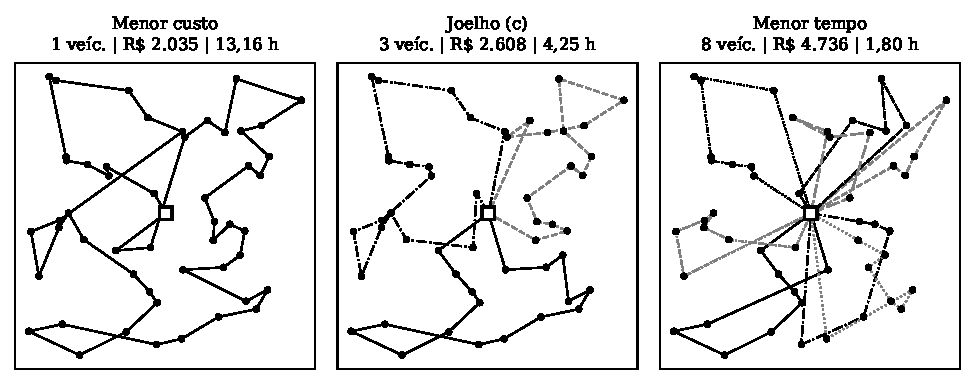
\includegraphics[width=1.0\linewidth]{figuras/fig_rotas.pdf}
  \caption{Rotas de três soluções da frente mediana. O quadrado é o depósito e cada estilo de linha representa um veículo.}
  \label{fig:rotas}
\end{figure}

\subsection{Discussão e limitações}\label{sec:disc}
\noindent A soma ponderada continua útil quando o decisor já conhece a importância relativa de custo e prazo; quando não conhece, a frente de Pareto torna explícito o preço de cada hora de antecipação. O estudo, porém, tem limitações: a instância é única, sintética e sem restrições de capacidade ou janelas de tempo, presentes na maioria das operações reais \citep{toth2014}; custos e velocidade são ilustrativos; os parâmetros não foram ajustados sistematicamente; a soma ponderada usou um único otimizador e guardou apenas uma solução por peso; e o NSGA-II foi aplicado sem busca local, que costuma ser decisiva em roteamento \citep{potvin2009}.


\section{Conclusão e Trabalhos Futuros}\label{sec:conc}
\noindent Este trabalho aplicou o NSGA-II a um problema sintético de roteamento com dois objetivos conflitantes, custo diário e tempo médio de entrega, e o comparou com a soma ponderada em 30 repetições. Com o mesmo orçamento, o NSGA-II obteve hipervolume de 0,851, contra 0,140. Com onze vezes mais avaliações, a soma ponderada chegou a 0,882, mas ofereceu em média 7,5 alternativas, contra 57,1 do NSGA-II, das quais, em média, 61\% continuam não dominadas diante das três abordagens e não são suportadas, ficando fora do alcance de qualquer combinação de pesos sobre a melhor frente conhecida. A frente permitiu escolher soluções por orçamento, por prazo e pelo ponto de joelho, mostrando ao gestor, em reais e em horas, o que se ganha e o que se perde em cada escolha.

Como trabalhos futuros, sugere-se: (i) incluir capacidade e janelas de tempo, com instâncias de referência da literatura; (ii) acrescentar busca local 2-opt ao NSGA-II para melhorar os extremos da frente; (iii) testar orçamentos maiores e outros algoritmos multiobjetivo; e (iv) aplicar o método a dados reais de uma operação de entregas.


\section*{Declaração de Uso de Inteligência Artificial}
\noindent Em conformidade com a Portaria CNPq nº 2.664/2026 e o Art. 12º do Manual de Normas de TCC da Universidade Tiradentes, os autores declaram que utilizaram a ferramenta de IA generativa Claude (Anthropic, modelo Claude Opus 5.5) nas seguintes etapas e finalidades: (i) \emph{levantamento bibliográfico}, para localizar e conferir os dados bibliográficos das referências, todas verificadas nas fontes originais; (ii) \emph{geração de código-fonte}, para escrever a primeira versão dos scripts do experimento, da análise estatística, das figuras e da verificação das tabelas, disponíveis no repositório indicado na Seção \ref{sec:impl}; (iii) \emph{redação preliminar}, para produzir um rascunho das seções do artigo, posteriormente revisado e ajustado pelos autores; (iv) \emph{tradução} do Resumo e das palavras-chave para o inglês; e (v) \emph{execução do experimento}, cujos scripts foram executados no ambiente da ferramenta, conforme a Seção \ref{sec:impl}. A ferramenta não foi usada para inventar ou estimar dados: todos os valores das tabelas e figuras resultam da execução do código e podem ser reproduzidos a partir do repositório. A autoria e a responsabilidade integral pelo conteúdo do trabalho permanecem dos autores.


\begin{thebibliography}{99}
\bibitem[Blank e Deb(2020)]{blank2020}
Blank, J. e Deb, K. (2020). pymoo: Multi-objective optimization in Python. \emph{IEEE Access}, 8:89497--89509.
\bibitem[Branke et~al.(2004)]{branke2004}
Branke, J., Deb, K., Dierolf, H. e Osswald, M. (2004). Finding knees in multi-objective optimization. In \emph{Parallel Problem Solving from Nature -- PPSN VIII}, volume 3242 de \emph{Lecture Notes in Computer Science}, p. 722--731. Springer.
\bibitem[Coello Coello et~al.(2007)]{coello2007}
Coello Coello, C. A., Lamont, G. B. e Van Veldhuizen, D. A. (2007). \emph{Evolutionary Algorithms for Solving Multi-Objective Problems}. Springer, 2ª edição.
\bibitem[Dantzig e Ramser(1959)]{dantzig1959}
Dantzig, G. B. e Ramser, J. H. (1959). The truck dispatching problem. \emph{Management Science}, 6(1):80--91.
\bibitem[Das e Dennis(1997)]{das1997}
Das, I. e Dennis, J. E. (1997). A closer look at drawbacks of minimizing weighted sums of objectives for Pareto set generation in multicriteria optimization problems. \emph{Structural Optimization}, 14(1):63--69.
\bibitem[Davis(1985)]{davis1985}
Davis, L. (1985). Applying adaptive algorithms to epistatic domains. In \emph{Proceedings of the 9th International Joint Conference on Artificial Intelligence (IJCAI)}, p. 162--164.
\bibitem[Deb(2001)]{deb2001}
Deb, K. (2001). \emph{Multi-Objective Optimization Using Evolutionary Algorithms}. John Wiley \& Sons.
\bibitem[Deb et~al.(2002)]{deb2002}
Deb, K., Pratap, A., Agarwal, S. e Meyarivan, T. (2002). A fast and elitist multiobjective genetic algorithm: NSGA-II. \emph{IEEE Transactions on Evolutionary Computation}, 6(2):182--197.
\bibitem[Garcia-Najera e Bullinaria(2010)]{garcia2010}
Garcia-Najera, A. e Bullinaria, J. A. (2010). Optimizing delivery time in multi-objective vehicle routing problems with time windows. In \emph{Parallel Problem Solving from Nature -- PPSN XI}, volume 6239 de \emph{Lecture Notes in Computer Science}, p. 51--60. Springer.
\bibitem[Garcia-Najera e Bullinaria(2011)]{garcia2011}
Garcia-Najera, A. e Bullinaria, J. A. (2011). An improved multi-objective evolutionary algorithm for the vehicle routing problem with time windows. \emph{Computers \& Operations Research}, 38(1):287--300.
\bibitem[Goldberg(1989)]{goldberg1989}
Goldberg, D. E. (1989). \emph{Genetic Algorithms in Search, Optimization, and Machine Learning}. Addison-Wesley.
\bibitem[Holland(1975)]{holland1975}
Holland, J. H. (1975). \emph{Adaptation in Natural and Artificial Systems}. University of Michigan Press.
\bibitem[Jozefowiez et~al.(2008)]{jozefowiez2008}
Jozefowiez, N., Semet, F. e Talbi, E.-G. (2008). Multi-objective vehicle routing problems. \emph{European Journal of Operational Research}, 189(2):293--309.
\bibitem[Mann e Whitney(1947)]{mann1947}
Mann, H. B. e Whitney, D. R. (1947). On a test of whether one of two random variables is stochastically larger than the other. \emph{The Annals of Mathematical Statistics}, 18(1):50--60.
\bibitem[Marler e Arora(2004)]{marler2004}
Marler, R. T. e Arora, J. S. (2004). Survey of multi-objective optimization methods for engineering. \emph{Structural and Multidisciplinary Optimization}, 26(6):369--395.
\bibitem[Miettinen(1999)]{miettinen1999}
Miettinen, K. (1999). \emph{Nonlinear Multiobjective Optimization}. Kluwer Academic Publishers.
\bibitem[Mundo Logística(2025)]{mundolog2025}
Mundo Logística (2025). Custo logístico do Brasil 2025 (dados do ILOS -- Instituto de Logística e Supply Chain). Disponível em: \url{https://mundologistica.com.br/noticias/custo-logistico-do-brasil-2025}. Acesso em: 30 out. 2026.
\bibitem[Potvin(2009)]{potvin2009}
Potvin, J.-Y. (2009). State-of-the art review -- evolutionary algorithms for vehicle routing. \emph{INFORMS Journal on Computing}, 21(4):518--548.
\bibitem[Toth e Vigo(2014)]{toth2014}
Toth, P. e Vigo, D., editores (2014). \emph{Vehicle Routing: Problems, Methods, and Applications}. SIAM, 2ª edição.
\bibitem[Zitzler e Thiele(1999)]{zitzler1999}
Zitzler, E. e Thiele, L. (1999). Multiobjective evolutionary algorithms: a comparative case study and the strength Pareto approach. \emph{IEEE Transactions on Evolutionary Computation}, 3(4):257--271.
\bibitem[Zitzler et~al.(2003)]{zitzler2003}
Zitzler, E., Thiele, L., Laumanns, M., Fonseca, C. M. e Grunert da Fonseca, V. (2003). Performance assessment of multiobjective optimizers: an analysis and review. \emph{IEEE Transactions on Evolutionary Computation}, 7(2):117--132.
\end{thebibliography}

\end{document}
